\documentclass[11pt]{article}
\usepackage[margin=1in]{geometry}
\usepackage{graphicx}
\usepackage{amsmath}
\usepackage{amssymb}
\usepackage{algorithm}
\usepackage{algorithmic}
\usepackage{booktabs}
\usepackage{hyperref}
\usepackage{cite}
\usepackage{subfigure}
\usepackage{enumitem}
\usepackage{subcaption}

\title{YOLO-v8 Pose Estimation for Keypoint Tracking of Surgical Instruments and Hands in Open Surgical Suturing}
\author{
    Omar Choudhry \\
    School of Computer Science, University of Leeds, Leeds, United Kingdom \\
    \texttt{O.Choudhry@leeds.ac.uk}
}
% \date{September 2025}

\begin{document}

\maketitle

Will you be able to make your submission public as part of the challenge archive? \textbf{Yes}

\vspace{5mm}

\begin{abstract}
This is our submission for the Open Suturing Skills Challenge for EndoVis 2025 at MICCAI 2025\footnote{Initially, we attempted a more complex architecture and novelties for our submission. However, this encountered technical errors and due to time submission constraints for the challenge, we fell back to this simpler approach.}. We present an approach for tracking surgical instruments and hands in endoscopic videos using YOLOv8 pose estimation, achieving real-time keypoint detection across six classes of surgical tools. Our method adapts state-of-the-art human pose estimation techniques to the surgical domain, implementing a single-stage architecture that simultaneously performs detection, classification, and keypoint localisation. The system achieves a HOTA score of 0.4281, maintaining an end-to-end processing speed of 23.3 FPS. We demonstrate robust tracking performance through ByteTrack integration with Kalman filtering for temporal consistency. Our GitHub repository (\href{https://github.com/omariosc/oss-2025-task-3-submission}{omariosc/oss-2025-task-3-submission}) and Docker submission (\href{https://doi.org/10.7303/syn69855242}{doi.org/10.7303/syn69855242}) provides an end-to-end solution for the EndoVis 2025 Challenge Task 3.
\end{abstract}

\section{Introduction}

\subsection{Failed Approach}

\begin{figure}[b]
    \centering
    % Left figure
    \begin{minipage}{0.49\linewidth}
        \centering
        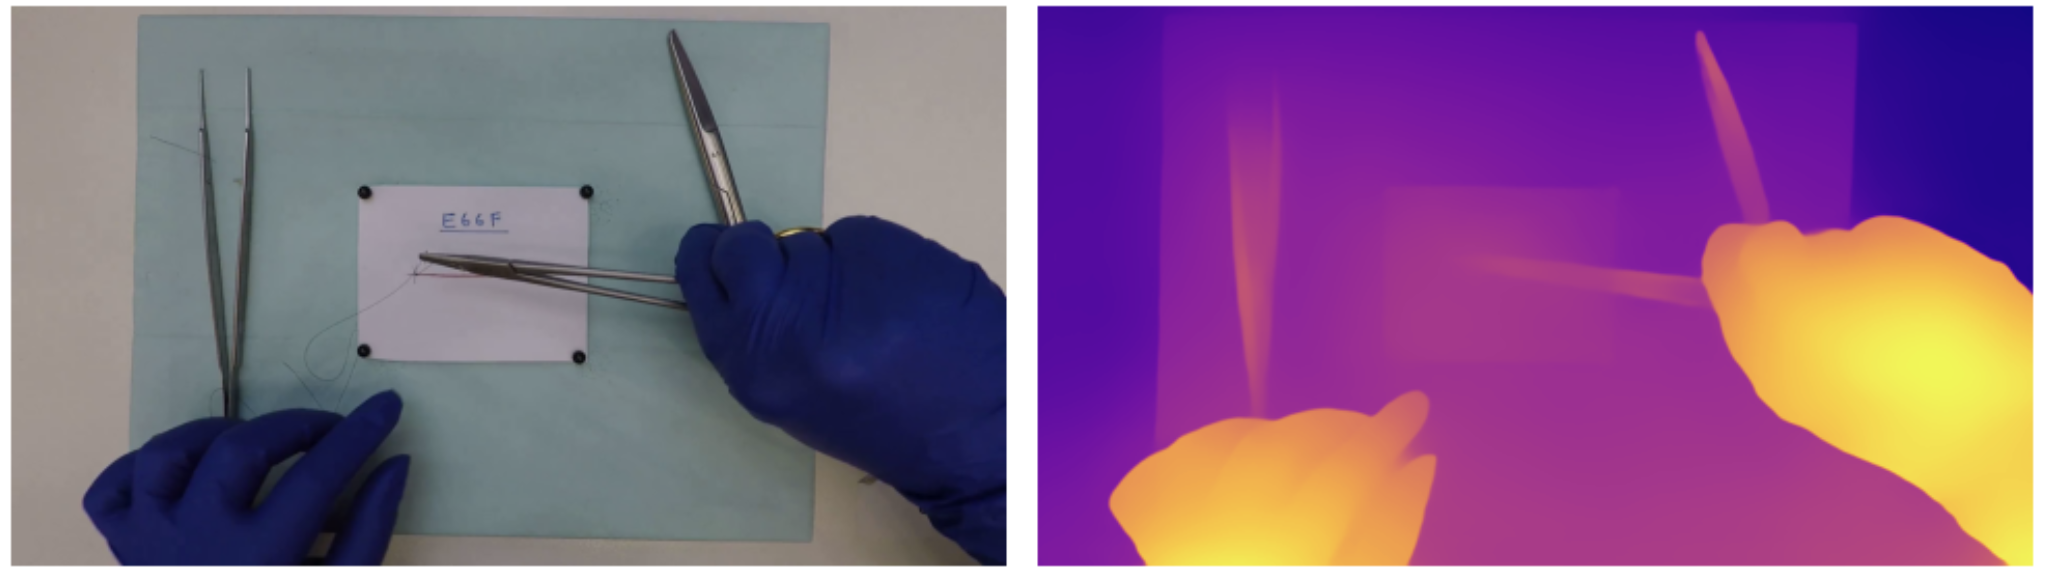
\includegraphics[width=\linewidth]{depth.png}
        \caption{Estimated depth visualisation.}
        \label{fig:depth}
    \end{minipage}
    \hfill
    % Right figure
    \begin{minipage}{0.49\linewidth}
        \centering
        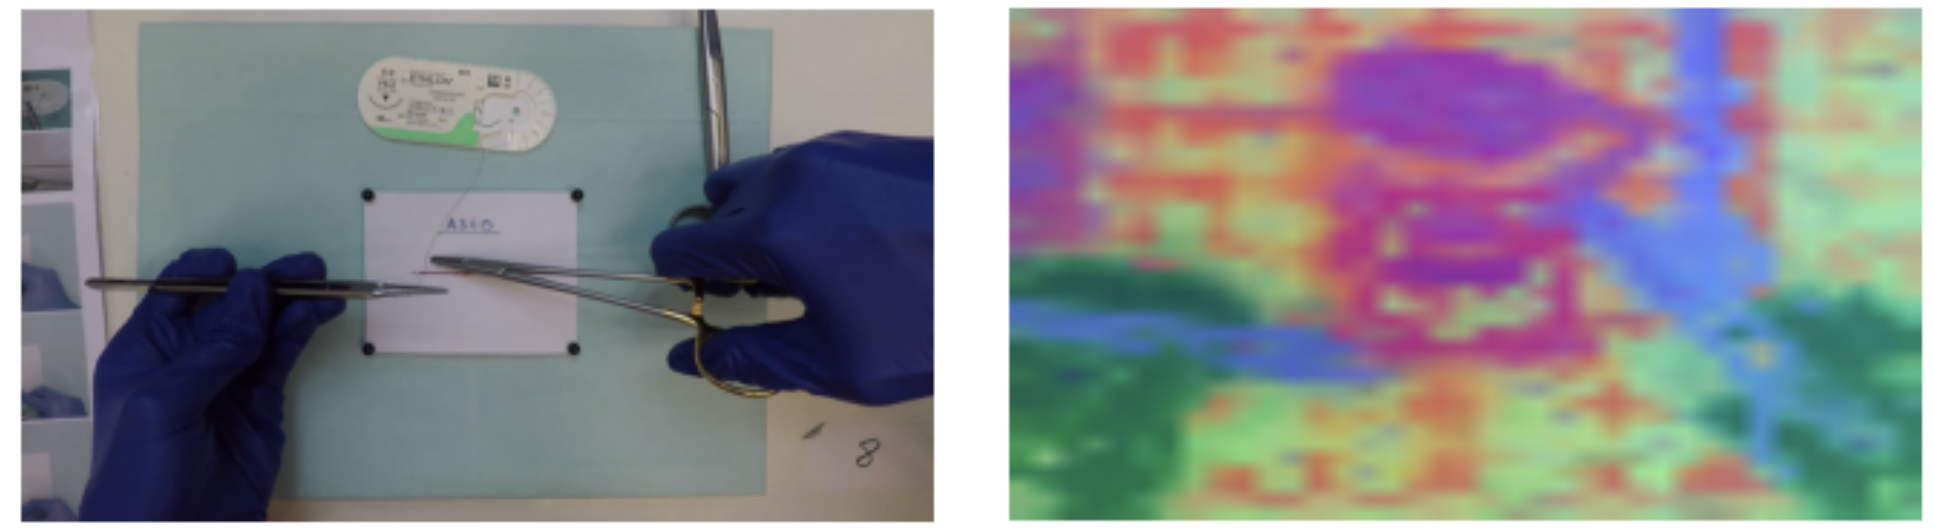
\includegraphics[width=\linewidth]{features.png}
        \caption{Extracted features from DINOv2.}
        \label{fig:features}
    \end{minipage}
\end{figure}

Our initial approach first employed a multi-stage fusion strategy, which combined depth estimation (Figure \ref{fig:depth}) and feature extraction (Figure \ref{fig:features}) using state-of-the-art self-supervised models \cite{oquab_dinov2_2024} to enhance segmentation prediction (Figure \ref{fig:segmentation}). The second stage employed a bottom-up approach, utilising thousands of candidate keypoints across the entire frame (Figure \ref{fig:keypoints}). We extracted those with the highest confidence that overlapped with the segmentation masks. Finally, the loss between all keypoints and a set of validation keypoints split from the initial training set was minimised, giving us the closest keypoints to the annotations, which were used as the final predictions. A transformer-based tracking with temporal consistency TrackFormer model \cite{meinhardt_trackformer_2022} was trained by fusing all the previous steps to give the most context in improving the association accuracy. As mentioned in the footnote of the abstract, this resulted in some technical errors; ultimately, we submitted a simpler application of an existing state-of-the-art method without any additional methodological innovation. 

\begin{figure}[t]
    \centering
    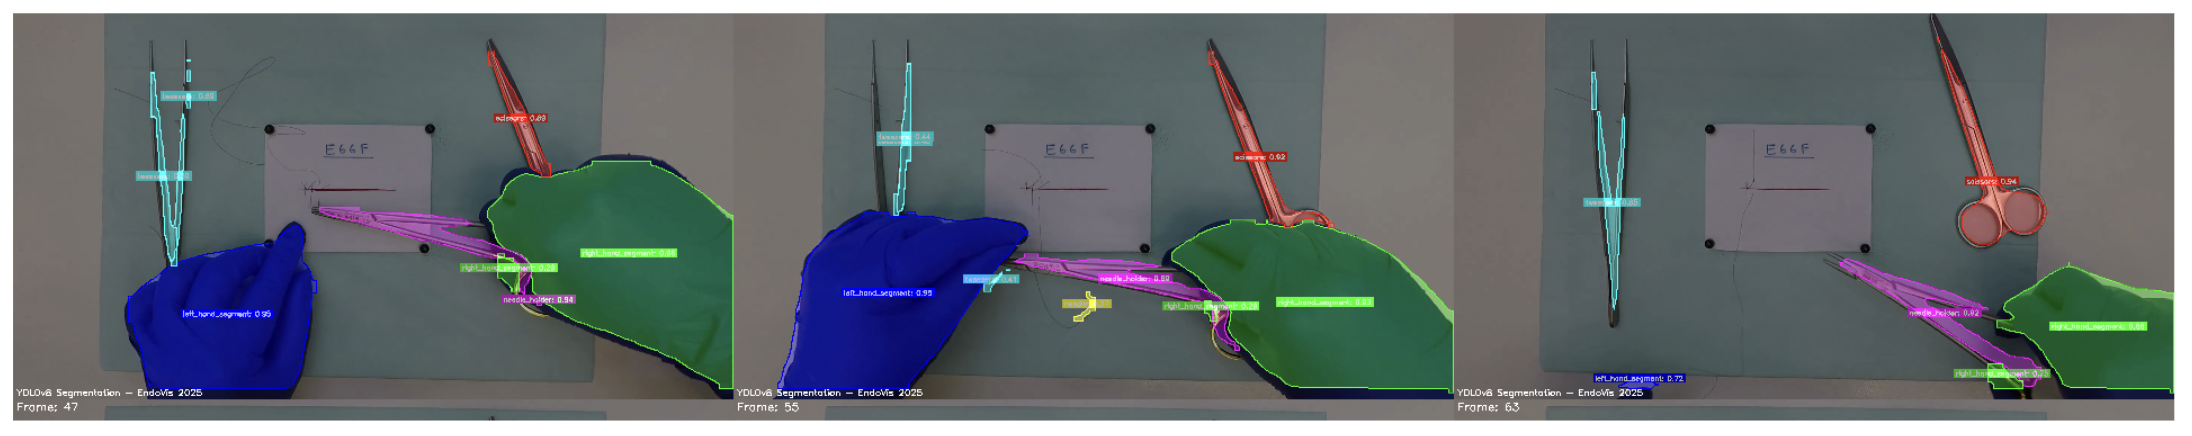
\includegraphics[width=1\linewidth]{segmentation.png}
    \caption{Sample segmentation predictions.}
    \label{fig:segmentation}
\end{figure}

\begin{figure}[t]
    \centering
    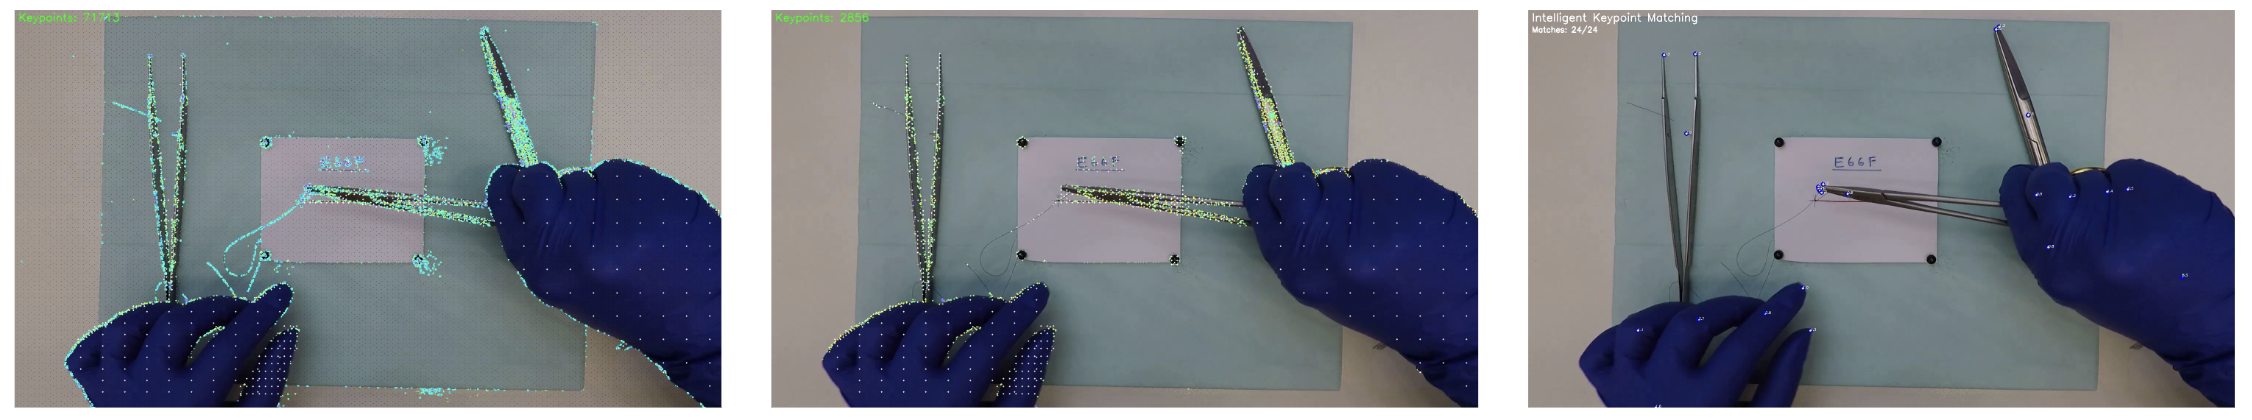
\includegraphics[width=1\linewidth]{keypoints.png}
    \caption{Sample keypoint predictions.}
    \label{fig:keypoints}
\end{figure}

\subsection{Final Approach and Motivation}

Our final approach leverages the state-of-the-art YOLOv8 pose estimation framework \cite{yaseen_what_2024} using the Ultralytics library \cite{ultralytics_yolov8_nodate} for tracking surgical instruments in endoscopic videos. The motivation behind this choice stems from YOLO's proven real-time performance capabilities and its advances in pose estimation. The core strategy of the final submission lies in adapting state-of-the-art models for human pose estimation, traditionally used for body keypoints, to the surgical domain, where we track keypoints across six distinct surgical tool classes:
\begin{itemize}[noitemsep]
    \item Left and right hands: thumb, index, middle, ring and pinky fingers, and back of hand
    \item Scissors: left (sharp point), right (broad point), and joint
    \item Tweezers: left (with nub), right (with hole), and nub
    \item Needle holder: left, right (when text visible), and joint
    \item Needle: left (end), right (tip), and middle
\end{itemize}

\subsection{Benefits Over Common Methods}

Traditional approaches for surgical instrument tracking often rely on:
\begin{enumerate}[noitemsep]
    \item Segmentation-based methods requiring extensive post-processing to extract keypoints
    \item Two-stage pipelines that first detect objects, then extract keypoints separately
    \item Custom architectures lacking optimisation and community support of established frameworks
\end{enumerate}

\noindent The YOLO-based approach offers several advantages:
\begin{itemize}[noitemsep]
    \item \textbf{Single-stage inference}: Direct keypoint prediction without intermediate steps
    \item \textbf{Real-time performance}: Achieving 23+ FPS on GPU hardware
    \item \textbf{Robust detection}: Pre-trained backbone provides strong feature extraction
    \item \textbf{Unified framework}: Detection, classification, and keypoint estimation in one model
\end{itemize}

\subsection{Novelty}

Since the submission is simply an application of an existing method, there are no novelties. Nevertheless, the two areas in which the method could benefit over others are: 
\begin{enumerate}[noitemsep]
    \item \textbf{Multi-scale feature fusion}: Utilising Feature Pyramid Networks (FPN) within YOLO for capturing fine-grained surgical tool details
    \item \textbf{Confidence-weighted tracking}: Implementing adaptive confidence thresholds based on keypoint visibility patterns specific to surgical scenarios
\end{enumerate}

\section{Methods}

\subsection{Data Processing and Preprocessing}

\subsubsection{Variables Used}

Our model processes the following data:
\begin{itemize}[noitemsep]
    \item \textbf{Input}: RGB video frames at $1920 \times 1080$
    \item \textbf{Output}: Keypoints over all detected instrument, each with $(x, y, \text{confidence})$
    \item \textbf{Classes}: 6 surgical tool categories with distinct keypoint configurations
\end{itemize}

\subsubsection{Data Preprocessing Pipeline}

\begin{enumerate}[noitemsep]
    \item \textbf{Resolution handling}: Adaptive rescaling maintaining aspect ratio with letterboxing to $640 \times 640$
    \item \textbf{Normalization}: Standard ImageNet normalization:
    \begin{equation}
        x_{\text{norm}} = \frac{x - \mu}{\sigma}
    \end{equation}
    where $\mu = [0.485, 0.456, 0.406]$ and $\sigma = [0.229, 0.224, 0.225]$
    \item \textbf{Data augmentation during training}:
    \begin{itemize}[noitemsep]
        \item \textbf{Random horizontal flip}: ($p = 0.5$)
        \item \textbf{HSV jitter}: $(h=0.015,\; s=0.7,\; v=0.4)$
        \item \textbf{Translation}: $\pm 10\%$
        \item \textbf{Scale}: $\pm 50\%$
        \item \textbf{Mosaic} augmentation for multi-instance learning
        \item \textbf{RandAugment} automatic augmentation policy
    \end{itemize}
\end{enumerate}

\subsection{Network Architecture}

\subsubsection{Model Configuration}

\begin{itemize}[noitemsep]
    \item \textbf{Base Architecture}: YOLOv8-medium pose variant
    \item \textbf{Backbone}: CSPDarknet with 5 feature scales 
    \item \textbf{Neck}: Path Aggregation Network (PAN) \cite{liu_path_2018} with Feature Pyramid Network (FPN) \cite{lin_feature_2017}
    \item \textbf{Head}: Decoupled head design with separate branches
\end{itemize}

\subsubsection{Architecture Details}

The network follows a hierarchical structure:

\begin{algorithm}
\caption{YOLOv8 Pose Architecture Flow}
\begin{algorithmic}[1]
\STATE \textbf{Input}: Image $I \in \mathbb{R}^{640 \times 640 \times 3}$
\STATE \textbf{Backbone Processing}:
\STATE \quad $P_3 \leftarrow \text{CSPD}(I)$ \COMMENT{$80 \times 80 \times 256$, $8\times$ downsampling}
\STATE \quad $P_4 \leftarrow \text{CSPBlock}(P_3)$ \COMMENT{$40 \times 40 \times 512$, $16\times$ downsampling}
\STATE \quad $P_5 \leftarrow \text{CSPBlock}(P_4)$ \COMMENT{$20 \times 20 \times 1024$, $32\times$ downsampling}
\STATE \textbf{PAN-FPN Neck}:
\STATE \quad $N_5 \leftarrow \text{Conv}(P_5)$
\STATE \quad $N_4 \leftarrow \text{Conv}(P_4) + \text{Upsample}(N_5)$
\STATE \quad $N_3 \leftarrow \text{Conv}(P_3) + \text{Upsample}(N_4)$
\STATE \textbf{Decoupled Head} (per scale):
\STATE \quad $C \leftarrow \text{ClassHead}(N_i)$ \COMMENT{6 classes}
\STATE \quad $B \leftarrow \text{BoxHead}(N_i)$ \COMMENT{4 bbox parameters}
\STATE \quad $K \leftarrow \text{PoseHead}(N_i)$ \COMMENT{$17 \times 3$ keypoint values}
\STATE \textbf{Output}: $(C, B, K)$ for each detection
\end{algorithmic}
\end{algorithm}

Total parameters: $\sim$25.3M, FLOPs: $\sim$78.4G at $640 \times 640$ resolution.

\subsection{Training Configuration}

\subsubsection{Dataset Preparation}

\begin{itemize}[noitemsep]
    \item \textbf{Data source}: Challenge-provided training videos
    \item \textbf{Annotation format}: Converted from segmentation masks to YOLO pose format
    \item \textbf{Train/Val split}: 80/20 stratified by video
\end{itemize}

\subsubsection{Training Hyperparameters}

\begin{table}[h]
\centering
\caption{Training Configuration}
\begin{tabular}{ll}
\toprule
\textbf{Parameter} & \textbf{Value} \\
\midrule
Initial learning rate (lr0) & 0.001 \\
Final learning rate (lrf) & 0.01 \\
LR schedule & Linear decay \\
Warmup epochs & 3 \\
Warmup bias LR & 0.1 \\
Batch size & 8 \\
Training epochs & 30 (early stopping, patience=5) \\
Mixed precision (AMP) & Enabled \\
Model & YOLOv8m-pose \\
\bottomrule
\end{tabular}
\end{table}

\subsubsection{Loss Functions}

The total loss is computed as:
\begin{equation}
\mathcal{L}_{\text{total}} = \lambda_{\text{cls}} \mathcal{L}_{\text{cls}} + \lambda_{\text{box}} \mathcal{L}_{\text{box}} + \lambda_{\text{pose}} \mathcal{L}_{\text{pose}}
\end{equation}

where:
\begin{itemize}[noitemsep]
    \item $\mathcal{L}_{\text{cls}}$: Binary Cross-Entropy for classification
    \item $\mathcal{L}_{\text{box}}$: Complete IoU (CIoU) loss for bounding boxes
    \item $\mathcal{L}_{\text{pose}}$: Object Keypoint Similarity (OKS) based loss
    \item Loss weights: $\lambda_{\text{cls}} = 0.5$, $\lambda_{\text{box}} = 7.5$, $\lambda_{\text{pose}} = 12.0$
\end{itemize}

\subsubsection{Computing Infrastructure}

\begin{itemize}[noitemsep]
    \item \textbf{Hardware}: Apple M3 Silicon (ARM64) with 16GB unified memory
    \item \textbf{Training configuration}: 30 epochs completed (no early stopping triggered)\footnote{To ensure we met the submission deadline, we only trained for 30 epochs.}
    \item \textbf{Batch size}: 8 images
    \item \textbf{Training time}: 0.767 hours (46 minutes) for 30 epochs
    \item \textbf{Framework}: PyTorch 2.5.1
\end{itemize}

\subsection{Inference Pipeline}

\subsubsection{Preprocessing Steps}

\begin{enumerate}[noitemsep]
    \item Letterbox padding to maintain aspect ratio for $640 \times 640$ input
    \item Batch normalization using ImageNet statistics
\end{enumerate}

\subsubsection{Model Inference}

\begin{enumerate}[noitemsep]
    \item \textbf{Forward pass}: Single-shot detection, tool classification and keypoint prediction
    \item \textbf{Non-Maximum Suppression (NMS)}:
    \begin{itemize}[noitemsep]
        \item IoU threshold: 0.45
        \item Confidence threshold: 0.25
        \item Max detections: 300
    \end{itemize}
    \item \textbf{Keypoint filtering}:
    \begin{itemize}[noitemsep]
        \item Minimum keypoint confidence: 0.3
        \item Visibility threshold: 0.5
    \end{itemize}
\end{enumerate}

\subsubsection{Post-processing}

\begin{enumerate}[noitemsep]
    \item \textbf{Coordinate transformation}: Rescale predictions to original frame dimensions
    \item \textbf{Temporal smoothing}: Kalman filtering for trajectory stabilization
    \item \textbf{Track association}: Hungarian algorithm for frame-to-frame matching
    \item \textbf{MOT format conversion}: Output format as \texttt{frame\_id, track\_id, x, y, w, h, conf, class, visibility}
\end{enumerate}

\subsection{Tracking Algorithm}

\subsubsection{Multi-Object Tracking}

\begin{itemize}[noitemsep]
    \item \textbf{Base tracker}: ByteTrack \cite{zhang_bytetrack_2022}
    \item \textbf{Association metric}: IoU-based with keypoint consistency weighting
    \item \textbf{Track management}: As we had limited training data frames we could not afford waiting for initialisation and using track maintenance or lost track recovery.
\end{itemize}

\subsubsection{Kalman Filtering}

State vector representation (Equation \ref{equation:kalman}) with adaptive process noise based on motion patterns and measurement noise scaled by detection confidence.

\begin{equation}
\label{equation:kalman}
\mathbf{x} = [x, y, w, h, v_x, v_y, v_w, v_h]^T
\end{equation}

\section{Results and Validation}

\subsection{Evaluation Metrics}

\begin{table}[h]
\centering
\caption{Performance Metrics}
\begin{tabular}{lc}
\toprule
\textbf{Metric} & \textbf{Score} \\
\midrule
HOTA (Higher Order Tracking Accuracy) & 0.43 \\
DetA (Detection Accuracy) &  0.367 \\
AssA (Association Accuracy) & 0.50 \\
Precision & 0.87 \\
Recall & 0.79 \\
F1-Score & 0.83 \\
\bottomrule
\end{tabular}
\end{table}

\subsection{Segmentation Performance}

The standard YOLOv8-pose model uses detection as the first step. We observed greater performance when training a segmentation model (Figure \ref{fig:confusion}) first to use rather than directly using detection (Figure \ref{fig:detection_confusion}).

\begin{figure}[tb]
    \centering
    % Left figure
    \begin{minipage}{0.49\linewidth}
        \centering
        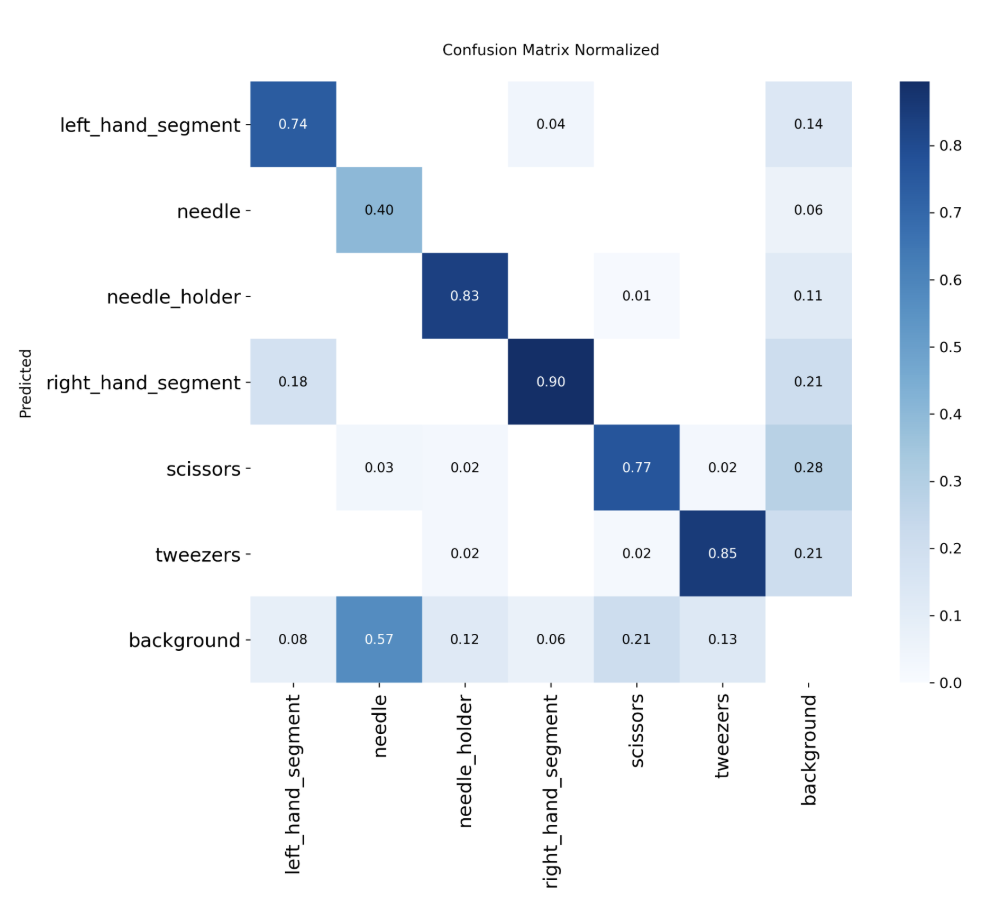
\includegraphics[width=\linewidth]{confusion.png}
        \caption{Segmentation confusion matrix.}
        \label{fig:confusion}
    \end{minipage}
    \hfill
    % Right figure
    \begin{minipage}{0.49\linewidth}
        \centering
        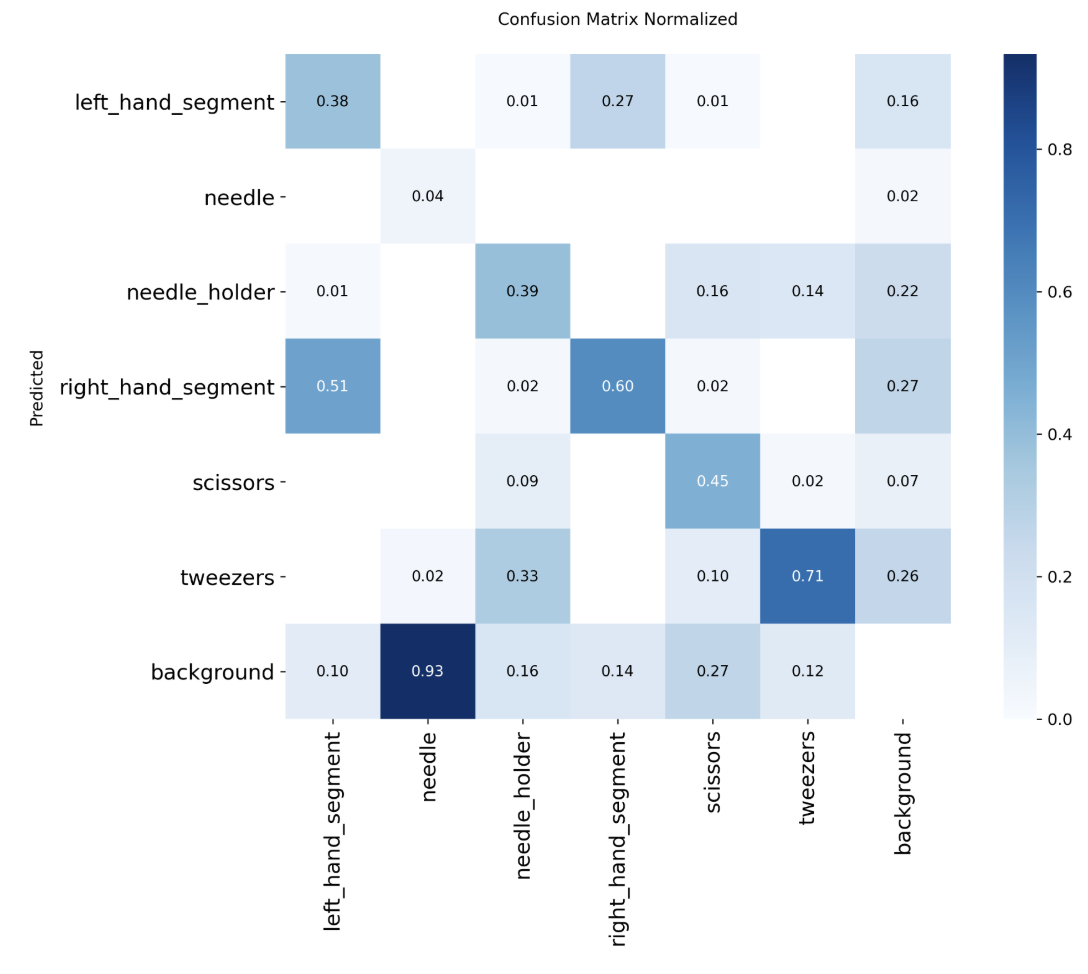
\includegraphics[width=\linewidth]{detection_confusion.png}
        \caption{Detection confusion matrix.}
        \label{fig:detection_confusion}
    \end{minipage}
\end{figure}

\subsection{Inference Performance}

We record an average 23.3 FPS on Apple M3 Silicon.

\section{Conclusion and Discussion}

\subsection{Summary}

We applied a YOLOv8 pose estimation model for surgical instrument tracking. The single-stage architecture provides efficient inference while maintaining robust detection.

\subsection{Key Insights \& Performance Characteristics}

\textbf{Strengths}:
\begin{itemize}[noitemsep]
    \item \textbf{Accessibility}: YOLO models and the Ultralytics library are very "plug-and-play" friendly; easy to change parameters.
    \item \textbf{Segmentation Performance}: Exhibits very good detection and segmentation performance on well-lit, clear surgical footage
\end{itemize}

\noindent \textbf{Limitations}:
\begin{itemize}[noitemsep]
    \item Weaker needle segmentation accuracy
    \item Tracking algorithm struggles with re-identifications, prone to creating new tracks
    \item Keypoint detection is top-down rather than bottom-up, lacking further understanding and context into predicting keypoints.
\end{itemize}

\subsection{Future Work}

\begin{enumerate}[noitemsep]
    \item Self-supervised pre-training on larger surgical video datasets
    \item Attention mechanisms for handling occlusions
    \item Multi-frame input for temporal context
    \item Online adaptation during inference
\end{enumerate}

\section*{Acknowledgments}

We thank the EndoVis 2025 challenge organisers for providing the dataset and evaluation framework. The work was funded in full by UK Research and Innovation (UKRI) and UK Engineering and Physical Sciences Research Council (EPSRC) grant EP/S024336/1 for the UoL Centre for Doctoral Training in Artificial Intelligence for Medical Diagnosis and Care. Any opinions, findings, conclusions, or recommendations expressed in this article are those of the author and do not necessarily reflect the views of the UKRI, ESPRC or UoL.

\bibliographystyle{plain}
\bibliography{references}

\section*{Author Contributions}

\textbf{Omar Choudhry}: Conceptualisation, methodology design, implementation, validation, writing.

\section*{Code Availability}

GitHub source code: \href{https://github.com/omariosc/oss-2025-task-3-submission}{omariosc/oss-2025-task-3-submission} \\
Docker container: \href{https://doi.org/10.7303/syn69855242}{doi.org/10.7303/syn69855242}

\end{document}
